\section{Cache solutions}

\subsection{Reversed proxy cache}

The figure \ref{fig:req_amount} shows the amount of requests and time that browser needs to make to generate a single VMO and  render a page. The browser needs to make more than 20 AJAX requests for a single page. The middleware was deployed on the local machine meaning that there is no latency bentween browser and middleware server. As can be seen, these are not optimistic numbers. The amount of requests is too high and computation have to be done on the both client and server sides. Several questions arises:
\begin{itemize}
	\item Is Redis a good caching layer for this project?
	\item Can Redis be replaced by something else? Maybe it would be better to use the configurational cache, represented by the web caches and control it through the http cache control headers.
\end{itemize}


\begin{figure}[h]
    \centering
	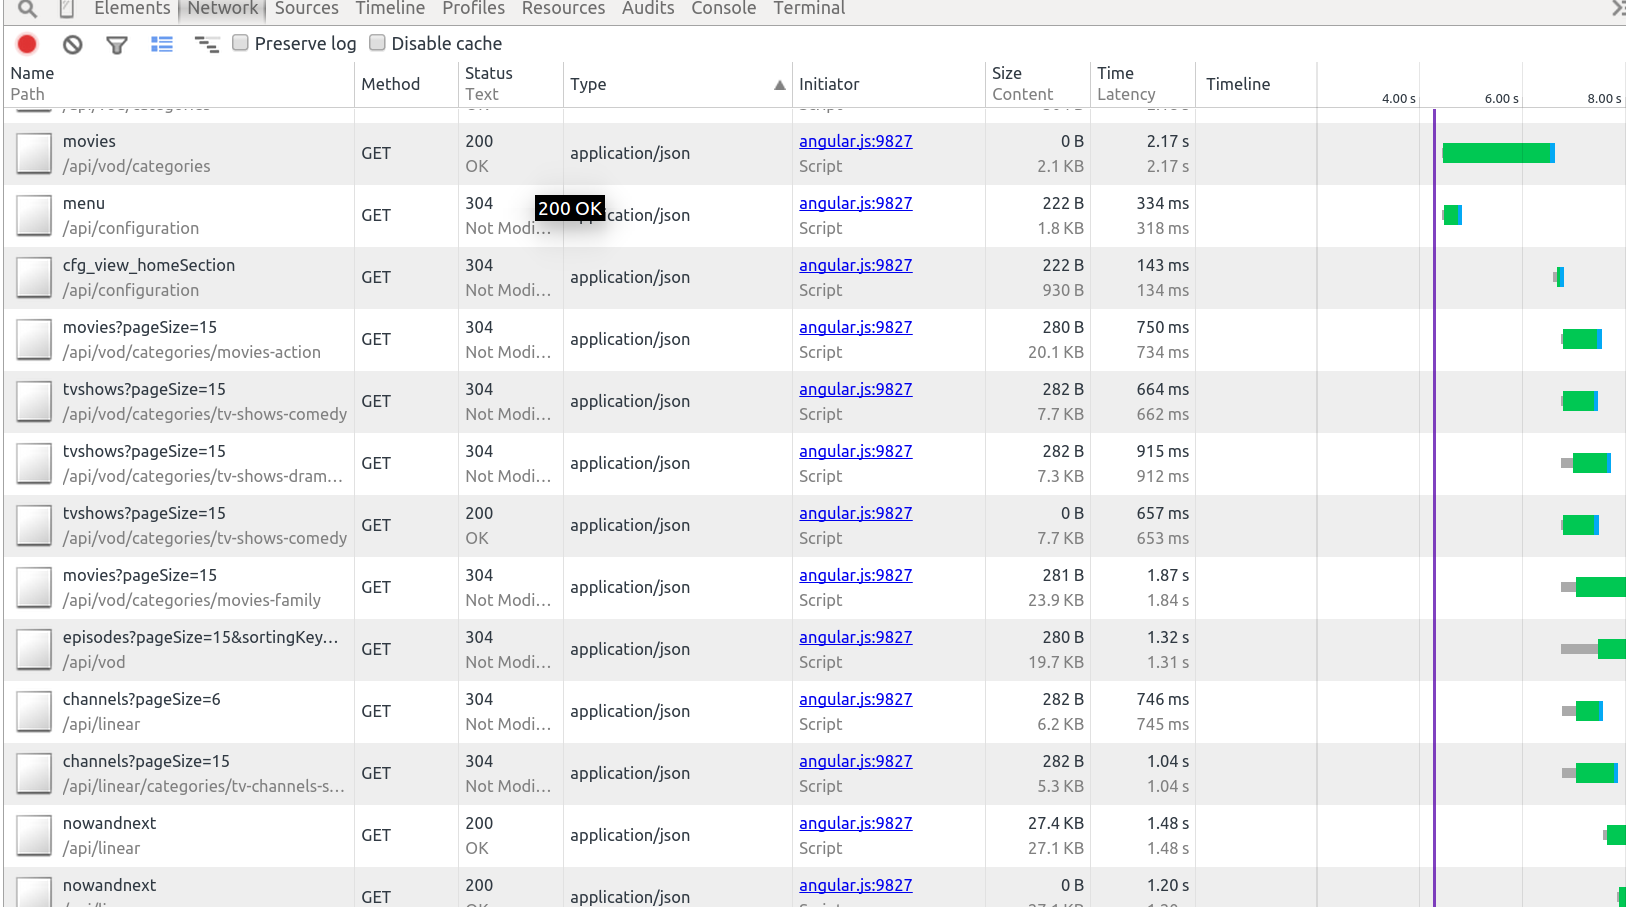
\includegraphics[width=\textwidth]{images/amount_of_requests.png}
    \caption{Example of page generation by browser}
    \label{fig:req_amount}
\end{figure}


Let’s consider system architecture using reversed proxy server instead of Redis cache. The client application will make http requests through the reversed proxy server. The proxy sever will decide if the content is stale or not and will act as a web cache. If the content is stale or non-cachable the proxy server will redirect request to the middleware server. Otherwise, it
will reply to the client application without touching the middleware server. The benefit of this solution is that instead of contacting server and than caching the object, the cache is contacted first and than the server. In theory it should give the performance and flexibility. The redis cache could be replaced by the Content Delivery Network solution in future.

% describe your solution on the top level

\subsection{Web cache selection}

The web cache for the project should satisfy several parameters:
\begin{itemize}
	\item Configurable. The client application sends requests both for DMOs and for writing user actions. The web cache should not cache the requests for writing user actions. The sessions still should be supported in order to write user actions. 
	\item Responsive, easy maintanable. The web cache should be deployed easily and provide statistics and internal logging. 
	\item High performance. The web cache should be transparent and must not increase the request time and latency if the cache object was not found locally. 
	% todo add more criterias
\end{itemize}

There are a many web cache solutions available both commercial and open source. For this project only open source solutions were considered. The initial candidates were: Squid, Varnish, Apache server with proxy module, Nginx server as a cachable reversed proxy and Apache Traffic Server.

The Squid server is a forward proxy server, but it can be configured as a reversed proxy server. Squid is preferably used for storing static content.

The Varnish was developed as a reversed proxy server from the beginning. It is fast, reliable and lightweigth. It uses Varnish Configuration Language(VCL) for configuration and describing the data workflow in cache. The VCL is translated to the C code and compiled to a shared object which is then dynamically linked into the server process. It is powerful tool that helps to set up Varnish as a dynamic reverse proxy server.

The Apache traffic server was developed by the Yahoo group and moved eventually to the Apache Incubator \cite{GuApacheTrafficUri}. According to Yahoo inc. Apache traffic server can handle more than 400TB of internet traffic per day and works as a forward as well as reversed proxy server. It has a growing community and continous improvement. The configuration is simple and consists of changing several files. All these, makes Apache traffic server a good candidate.  

Other solutions(Nginx and Apache server) was not developed to be proxy servers, but have additional modules that one can install and configure. They are not well-configured and work worst than solutions described above \cite{GuApacheTrafficUri}[change].

The thorough comparison and performance evaluation of Varnish and Apache Traffic Server could be found in \cite{VarnApacheReverse}.    

%TODO make a benchmarking analysis of the open web proxy caches
%TODO update the report, insert thate results about benchmarking and selection

\subsection{Web cache configuration}

Before performing execution and comparative study reversed proxy servers should be properly configured. They should aggregate and store requests that contain public data and skip analytical requests and requests with private user information(e.g. payments).

Proxy servers should also work with http sessions. Usually, when session is specified(the set-cookie http header included in the server response), proxy servers are transparent, meaning they are skipping these requests and not store them in memory. As was described in previous chapters, the metadata server uses http session for analytical purposes. It means that even anonymous users will have the unique session. 

In order to solve the problem, the Varnish was configured to replace Cookie header with X-Cookie header. This gives the possibility for Varnish to store the requests and still have the analytical requests available. The metadata server was modified in order to treat X-Cookie header as a Cookie header.   

The Varnish configuration is presented in Appendix A.

The Apache traffic server did not require a specific configuration. 


\newpage